\documentclass{article}

% preambulo:
\usepackage[utf8]{inputenc}
% caracteres utf8 (tildes, enie) sin tener que usar comandos

\usepackage[spanish, es-tabla, es-nodecimaldot]{babel} 
% texto automatico en espaniol
% "tabla" en vez de "cuadro"
% no reemplaza puntos decimales por comas

%% NO AGREGAR PAQUETES ANTES DE ESTO, ES IMPORTANTE QUE BABEL ESTE PRIMERO

%%%%%%%%%%%%%%%%%%%%%%%%%%%%%%%%%
%% PAQUETES EXTRA %%%%%%%%%%%%%%%
%%%%%%%%%%%%%%%%%%%%%%%%%%%%%%%%%

\usepackage{subfiles}

\usepackage{amsmath} % PAQUETES DE MATEMATICA
\usepackage{amsfonts}
\usepackage{amssymb}


\usepackage{steinmetz} % comando \phase{}
\usepackage{units} % permite usar nicefrac
\usepackage{graphicx} % importar imagenes
\usepackage{float} % posicion H para floats
\usepackage[colorinlistoftodos]{todonotes}


\usepackage[a4paper]{geometry} 
% margenes correctos en subarchivos

\setlength{\parindent}{10pt}			%cuanta sangria al principio de un parrafo
\usepackage{indentfirst}				%pone sangria al primer parrafo de una seccion


\usepackage{fancyhdr}
\usepackage{lscape}
\usepackage{units}

\geometry{top=2.5cm, bottom=2.0cm, left=2.25cm, right=2.25cm}

\lhead{Elec Air}
\chead{Placa Tiempo Universal}
\rhead{Datasheet}
\renewcommand{\headrulewidth}{1pt}
\renewcommand{\footrulewidth}{1pt}

\pagestyle{fancy}



%%%%%%%%%%%%%%%%%%%%%%%%%%%%%%%%%%%%%%%%%%%%%%%%%%%%%%%%%%%
%% NO AGREGAR PAQUETES DESPUES DE ESTO, ES IMPORTANTE QUE HYPERREF ESTE ULTIMO
\usepackage[hidelinks]{hyperref} % hipervinculos sin cajitas rojas



\begin{document}

\section*{Placa de Tiempo Universal - Elec Air}

\subsection*{Placa Esquemática}

\begin{figure}[H]
\centering
%\includegraphics[width=0.8\linewidth]{images/placa.jpg}
\end{figure}

\subsection*{Descripción}

\large{Placa universal de tiempos adaptable a tres circuitos de encendido, tanto por chispa, por incandescente, y por válvula electrónica. Se adjuntan los planos de conexionado correspondientes en las secciones siguientes.}

\subsection*{Equipos compatibles}
\large{
\begin{itemize}
\item Calefactores GOODMAN
\item Calefactores CARRIER
\item Calefactores GOODMAN-CARRIER
\item Calefactores GOODMAN-SURREY
\item Calefactores (Ex) CONFORMAKER
\item Calefactores BGH
\item Calefactores LENNOX
\end{itemize}
}

\newpage

\subsection*{Circuito eléctrico - Versión por chispa}

\begin{figure}[H]
\centering

\includegraphics[width=0.65\linewidth]{images/PlacaTiempo_PlanoV623.png}
\end{figure}

\newpage

\subsection*{Tiempos de Marcha - Parada}
\begin{itemize}
\item FAN en G:
\begin{itemize}
\item ON - 10 Seg
\item OFF - 3 Seg
\end{itemize}

\item EXT. DE GAS en W:
\begin{itemize}
\item ON - 10 Seg
\item OFF - 20 Seg
\end{itemize}

\item FAN en W:
\begin{itemize}
\item ON - 20 Seg luego de luz verde fija
\item OFF - 3 Min luego de parada señal W
\end{itemize}

\item SENSOR DE VACÍO:
\begin{itemize}
\item OFF - 7 Seg
\end{itemize}
\end{itemize}

\subsection*{Código de Fallas}
\begin{itemize}
\item LED VERDE FIJO: Operación normal
\item LED VERDE TITILANTE CADA 0.5 SEG.: Espera señal de válvula
\item LED ROJO TITILANTE CADA 0.5 SEG.: Límite abierto
\item LED VERDE/ROJO ALTERNANDO CADA 0.5 SEG.: Sensor de vacío en corto antes de iniciar secuencia
\item LED ROJO FIJO: Placa bloqueada por falla externa de límite abierto 3 veces
\end{itemize}

\subsection*{NOTA IMPORTANTE}
\begin{itemize}
\item DEBE conectarse el sensor de vacío en el circuito. Este puede reemplazarse por llave centrífuga NA, ubicada en motores de extracción de gases.
\item DEBE conectarse el calefactor con jabalina a tierra.
\item La placa queda fuera de garantía por mal conexionado.
\end{itemize}

\subsection*{Notas de uso}
Los momentos de funcionamiento de la placa de tiempos están superditados a las funciones de encendido generadas por la placa de chispa. Éstas están dadas por el fabricante de esa marca.\par Si la placa de encendido \textbf{no} funciona, la placa de tiempo \textbf{no} realiza su ciclo de programa por seguridad.

\newpage

\subsection*{Circuito eléctrico - Versión por chispa (con Piloto)}

\begin{figure}[H]
\centering
\includegraphics[width=0.65\linewidth]{images/PlacaTiempo_PlanoV623ConPiloto.png}
\end{figure}

\newpage

\subsection*{Tiempos de Marcha - Parada}
\begin{itemize}
\item FAN en G:
\begin{itemize}
\item ON - 10 Seg
\item OFF - 3 Seg
\end{itemize}

\item EXT. DE GAS en W:
\begin{itemize}
\item ON - 10 Seg
\item OFF - 20 Seg
\end{itemize}

\item FAN en W:
\begin{itemize}
\item ON - 20 Seg luego de luz verde fija
\item OFF - 3 Min luego de parada señal W
\end{itemize}

\item SENSOR DE VACÍO:
\begin{itemize}
\item OFF - 7 Seg
\end{itemize}
\end{itemize}

\subsection*{Código de Fallas}
\begin{itemize}
\item LED VERDE FIJO: Operación normal
\item LED VERDE TITILANTE CADA 0.5 SEG.: Espera señal de válvula
\item LED ROJO TITILANTE CADA 0.5 SEG.: Límite abierto
\item LED VERDE/ROJO ALTERNANDO CADA 0.5 SEG.: Sensor de vacío en corto antes de iniciar secuencia
\item LED ROJO FIJO: Placa bloqueada por falla externa de límite abierto 3 veces
\end{itemize}

\subsection*{NOTA IMPORTANTE}
\begin{itemize}
\item $\cdot \cdot \cdot \cdot \cdot$ Opcional con Piloto
\item DEBE conectarse el sensor de vacío en el circuito. Este puede reemplazarse por llave centrífuga NA, ubicada en motores de extracción de gases.
\item DEBE conectarse el calefactor con jabalina a tierra.
\item La placa queda fuera de garantía por mal conexionado.
\end{itemize}

\subsection*{Notas de uso}
Los momentos de funcionamiento de la placa de tiempos están superditados a las funciones de encendido generadas por la placa de chispa. Éstas están dadas por el fabricante de esa marca.\par Si la placa de encendido \textbf{no} funciona, la placa de tiempo \textbf{no} realiza su ciclo de programa por seguridad.
\newpage

\newpage

\subsection*{Circuito eléctrico - Versión por superficie caliente}

\begin{figure}[H]
\centering

\includegraphics[width=0.65\linewidth]{images/PlacaTiempo_PlanoFenwallV623.png}
\end{figure}

\newpage

\subsection*{Tiempos de Marcha - Parada}
\begin{itemize}
\item FAN en G:
\begin{itemize}
\item ON - 10 Seg
\item OFF - 3 Seg
\end{itemize}

\item EXT. DE GAS en W:
\begin{itemize}
\item ON - 10 Seg
\item OFF - 20 Seg
\end{itemize}

\item FAN en W:
\begin{itemize}
\item ON - 20 Seg luego de luz verde fija
\item OFF - 3 Min luego de parada señal W
\end{itemize}

\item SENSOR DE VACÍO:
\begin{itemize}
\item OFF - 7 Seg
\end{itemize}
\end{itemize}

\subsection*{Código de Fallas}
\begin{itemize}
\item LED VERDE FIJO: Operación normal
\item LED VERDE TITILANTE CADA 0.5 SEG.: Espera señal de válvula
\item LED ROJO TITILANTE CADA 0.5 SEG.: Límite abierto
\item LED VERDE/ROJO ALTERNANDO CADA 0.5 SEG.: Sensor de vacío en corto antes de iniciar secuencia
\item LED ROJO FIJO: Placa bloqueada por falla externa de límite abierto 3 veces
\end{itemize}

\subsection*{NOTA IMPORTANTE}
\begin{itemize}
\item DEBE conectarse el sensor de vacío en el circuito. Este puede reemplazarse por llave centrífuga NA, ubicada en motores de extracción de gases.
\item DEBE conectarse el calefactor con jabalina a tierra.
\item La placa queda fuera de garantía por mal conexionado.
\end{itemize}

\subsection*{Notas de uso}
Los momentos de funcionamiento de la placa de tiempos están superditados a las funciones de encendido generadas por la placa de chispa. Éstas están dadas por el fabricante de esa marca.\par Si la placa de encendido \textbf{no} funciona, la placa de tiempo \textbf{no} realiza su ciclo de programa por seguridad.

\newpage

\subsection*{Circuito eléctrico - Versión por válvula de control electrónico}

\begin{figure}[H]
\centering
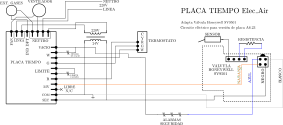
\includegraphics[width=0.65\linewidth]{images/PlacaTiempo_PlanoValvulaV623.png}
\end{figure}

\newpage

\subsection*{Tiempos de Marcha - Parada}
\begin{itemize}
\item FAN en G:
\begin{itemize}
\item ON - 10 Seg
\item OFF - 3 Seg
\end{itemize}

\item EXT. DE GAS en W:
\begin{itemize}
\item ON - 10 Seg
\item OFF - 20 Seg
\end{itemize}

\item FAN en W:
\begin{itemize}
\item ON - 20 Seg luego de luz verde fija
\item OFF - 3 Min luego de parada señal W
\end{itemize}

\item SENSOR DE VACÍO:
\begin{itemize}
\item OFF - 7 Seg
\end{itemize}
\end{itemize}

\subsection*{Código de Fallas}
\begin{itemize}
\item LED VERDE FIJO: Operación normal
\item LED VERDE TITILANTE CADA 0.5 SEG.: Espera señal de válvula
\item LED ROJO TITILANTE CADA 0.5 SEG.: Límite abierto
\item LED VERDE/ROJO ALTERNANDO CADA 0.5 SEG.: Sensor de vacío en corto antes de iniciar secuencia
\item LED ROJO FIJO: Placa bloqueada por falla externa de límite abierto 3 veces
\end{itemize}

\subsection*{NOTA IMPORTANTE}
\begin{itemize}
\item DEBE conectarse el sensor de vacío en el circuito. Este puede reemplazarse por llave centrífuga NA, ubicada en motores de extracción de gases.
\item DEBE conectarse el calefactor con jabalina a tierra.
\item La placa queda fuera de garantía por mal conexionado.
\end{itemize}

\subsection*{Notas de uso}
Los momentos de funcionamiento de la placa de tiempos están superditados a las funciones de encendido generadas por la placa de chispa. Éstas están dadas por el fabricante de esa marca.\par Si la placa de encendido \textbf{no} funciona, la placa de tiempo \textbf{no} realiza su ciclo de programa por seguridad.

\end{document}
